\section{Primary Producer Service}\label{sec:PrimaryProducer}\index{primary producer}

\subsection{Description}

Primary Producer resources are created by the Primary Producer Service
at the request of a user who wishes to publish tuples into to one or
more tables in a virtual database\index{virtual database}.
The principal components of a
Primary Producer resource are shown in the picture below. They contain
tuple stores\index{tuple store} to hold tuples inserted by the user,
and they have an SQL query processor to run consumer queries against
their tuple stores. They are the primary source of data in a virtual
database. They all support continuous queries, and can be configured
to support any combination of latest and history queries as well.

\begin{center}
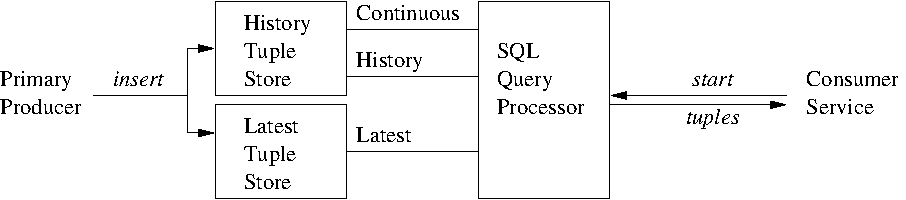
\includegraphics[width=145mm]{pp_detail}
\end{center}

The Primary Producer Service is responsible for authenticating all users and
services that connect to it, and for authorizing all operations and all requests
to access its tuple stores, as specified in chapter~\ref{sec:Security}.

\subsection{Interface}

\subsubsection{User Interface}

\begin{method}{createPrimaryProducer}
\inpar{xsd:boolean isHistory}{If history queries are supported}
\inpar{xsd:boolean isLatest}{If latest queries are supported}
\inpar{xsd:string type} {DATABASE or MEMORY}
\inpar{xsd:string logicalName}{The logical name should not be
be specified for type MEMORY. For type DATABASE it is optional.} 
\outhead{Tuple(1..1)}{}
\outpar{xsd:int connectionId}{connectionId of new Primary Producer resource.} 
\desc
Creates a new Primary Producer resource and returns its endpoint. The
Primary Producer is not added to a Registry until
\textit{declareTable} is called. The user cannot prevent Primary
Producers from supporting continuous queries, but support for latest
and/or history queries is optional. Primary Producers can use any type
of storage, regardless of the query types they support. Tuple stores can be
made permanent by providing a \textit{logical name} for the tuple store as
described in \ref{sec:PrimaryProducerTupleStores}. The termination interval is
described in \ref{sec:PrimaryProducerCreating}.
\end{method}

\begin{method}{declareTable}
\inpar{xsd:int connectionId}{Primary Producer resource identifier.}
\inpar{xsd:string tableName}{VDBTable to register.}
\inpar{xsd:string predicate}{Producer's predicate.}
\inpar{xsd:int hrpSec}{History Retention Period in seconds.}
\inpar{xsd:int lrpSec}{Latest Retention Period in seconds.}
\OK
\desc
Adds a table to the list of tables to which this producer may publish tuples,
as described in \ref{sec:PrimaryProducerDeclaring} below. The table name must
have an explicit virtual database name prefix (separated from it by a dot).
The format of the predicate is specified in \ref{sec:SQLPredicates}, and
the retention periods are described in \ref{sec:PrimaryProducerRemoving} (the 
latest retention period can be overridden in \textit{insert}). 
\end{method}

\begin{method}{insert}
\inpar{xsd:int connectionId}{Primary Producer resource identifier.}
\inpar{xsd:string insert}{SQL INSERT statement.}
\inpar{xsd:int(0..1) lrpSec}{Latest Retention Period in seconds.}
\OK
\desc
Inserts one or more tuples into a primary producer resource's tuple stores, as
described in \ref{sec:PrimaryProducerInserting}. The format of the insert
statement is specified in \ref{sec:SQLInsert}; as with \textit{declareTable},
the table name must have an explicit virtual database name prefix. Inserted
tuples must match the producer's predicate and the table schema or they will be
rejected. If the latest retention period is omitted, the default specified in
the call to \textit{declareTable} will be used. If a tuple is found to be invalid or cannot
be inserted for any reason, the operation will stop and throw an
RGMAException indicating the number of tuples successfully inserted in
its \textit{numSuccessfulOps} field (those tuples will remain in the tuple
stores).
\end{method}

\begin{method}{getLatestRetentionPeriod}
\inpar{xsd:int connectionId}{Primary Producer resource identifier.}
\inpar{xsd:string tableName}{VDBTable name.}
\outhead{Tuple(1..1)}{}
\outpar{xsd:int hrpSec}{Latest Retention Period in seconds.}
\desc Returns a Primary Producer resource's declared Latest Retention Period for
a given table.
\end{method}

See also the common producer service operations:
getHistoryRetentionperiod~\ref{op:getHistoryRetentionPeriod}.

See also the common resource management service operations:
close~\ref{op:close} and
destroy~\ref{op:destroy}.

See also the operation common to all services:
getProperty~\ref{op:getProperty}.

\subsubsection{System Interface}

See  the common producer service operations:
start~\ref{op:start} and abort~\ref{op:producerabort}.

See the common resource management service operation:
ping~\ref{op:resourceping}.

\subsection{Details}
\subsubsection{Creating and destroying Primary Producers}\label{sec:PrimaryProducerCreating}

A new Primary Producer Resource is created when a user calls the
\textit{createPrimaryProducer} operation and is destroyed when the
user calls the \textit{close} or \textit{destroy} operations. The
special processing for \textit{close} is desribed below. In addition,
if the service does not hear from the user for a period exceeding the
\textit{termination interval}\index{termination interval}, the service
will initiate a \textit{close} operation on the resource. A call to
any user operation on the resource is sufficient to keep it alive.

\subsubsection{Tuple stores}\label{sec:PrimaryProducerTupleStores}\index{tuple store}

The Primary Producer's history and latest tuple stores were described in 
\ref{sec:BackgroundTupleManagement}. They may be physically in memory or 
database storage. The memory storage may also make use of an RDBMS (typically 
memory resident) but is transient. A single producer uses 
only one type of storage for all types of queries that it supports.

The Primary and Secondary Producer services only uses stores created and 
managed by themselves. Tuple stores are normally temporary and are destroyed 
along with the producer resource, but users can make atuple store with database 
storage permanent by specifying a \textit{logical name} for the tuple store 
when they create a new Primary (or Secondary) producer. If the service is 
running in secure mode, the user's Distinguished Name (DN) is prefixed to the 
logical name. In insecure mode, the user must make the name unique within the 
service by some other means. Permanent tuple stores are not destroyed when a 
producer resource is destroyed, so they can be re-used by creating a new 
producer and naming the same store, provided there are no other producers using 
it already. The user can then re-declare any table that is already in the store 
(with a compatible predicate - see \ref{sec:SQLPredicates}) and any existing 
tuples will be automatically recovered. The names and some information about 
tuple stores can be obtained by calling \textit{listTupleStores}. Permanent tuple 
stores are deleted by calling \textit{dropTupleStore}. R-GMA only allows the 
the \textit{owners} of existing tuple stores to re-use or list them.

\subsubsection{Declaring tables}\label{sec:PrimaryProducerDeclaring}\index{declare table}

Producers must declare their intention to publish to a table by calling
\textit{declareTable} before they can insert tuples. The table definition must
already exist in the schema (see \ref{sec:SQLCreateTable}). The Primary
Producer Service obtains the table
definition from the schema by calling \textit{getFullTableDetails} and creates
the corresponding table in the resource's tuple stores (or if it already exists
in a named tuple store, checks its structure). If the
schema specifies that the table should be indexed, the producer creates the
indexes if possible, and also indexes the \textit{RgmaTimestamp} column (see
below).  It then registers the producer as a publisher for
that table, by calling the registry's \textit{registerProducerTable} operation.
The service must be ready to service consumer queries against the resource's
tuple stores as soon as this notification is sent.
This registry operation returns a list of any relevant continuous consumers
and the producer service must send an \textit{addProducer} message to each of
them to notify them about the new producer.
The producer service will also periodically re-send the
\textit{registerProducerTable} to the registry on the user's behalf, to
maintain the producer's entries in the registry throughout its lifetime. The
list of consumers returned is used to help check that consumers are still alive
(see \ref{sec:PrimaryProducerStoppingQueries}).
The user can declare more than one table in a single producer, and these can
even be in different virtual databases. All the tables are treated
independently by the producer service, except for processing ``join'' queries.

\subsubsection{Inserting tuples}\label{sec:PrimaryProducerInserting}\index{insert}

Tuples are inserted into the producer service's tuple storage by calling the
\textit{insert} or \textit{insertList} operations. They are checked for type
against the schema, and for content against the producer's declared predicate.
The following metadata is added to each tuple by the service:

\bigskip\begin{tabular}{llp{95mm}}
MeasurementDate&DATE&This and the next column will be supported for a while for
backward compatibility. At some stage they will be turned into user columns so
that they can be eliminated.\\
MeasurementTime&TIME&See above\\
RgmaTimestamp&TIMESTAMP(9)&
UTC tuple time-stamp: only added by R-GMA if not already filled in by the user;
those added by R-GMA will only have a resolution of 1ms
(see \ref{sec:SQLDataTypes} for the format of a TIMESTAMP)\\
RgmaLRT&TIMESTAMP(6)&
UTC Latest Retention Time (see below)\\
RgmaOriginalServer&VARCHAR(255)&
Hostname (including domain name) of server publishing the information.\\
RgmaOriginalClient&VARCHAR(255)&
Hostname (including domain name) of client publishing the information.\\
\end{tabular}\par\bigskip

Tuples are inserted to the tuple stores and streamed to subscribed consumers
as described in \ref{sec:BackgroundTupleManagement}. If one of the producer's
tuple stores fills up, the service temporarily blocks inserts by returning
an RGMABufferFullException until tuples expire and can be removed, as
described below.

A Producer making use of a named tuple store should avoid sending tuples that
have already been sent by another producer that used the store previously.

\subsubsection{Removing tuples}\label{sec:PrimaryProducerRemoving}\index{History Retention Period}

The user must set a \textit{History Retention Period (HRP)} and a 
\textit{Latest Retention Period (LRP)} for each declared table. The HRP is 
recorded in the registry indicating to the mediator the maximum age of tuples 
it guarantees to maintain in its history tuple store. The Primary Producer 
Service adjusts the HRP it sends to the registry to take account of the actual 
age of its history tuple store (which will be very short for a new producer), 
and updates it in the periodic calls to \textit{registerProducerTable} up to 
the value set by the user as time progresses. The LRP\index{Latest Retention 
Period} is used to calculate a \textit{Latest Retention Time 
(LRT)}\index{Latest Retention Time}\index{LRT|see{Latest Retention Time}} for 
each tuple by adding it to the tuple's RgmaTimestamp (the table-default LRP may be 
overridden in each call to \textit{insert}). The LRT is written into the 
tuple's metadata because Secondary Producers must also respect it. The two 
retention periods are independent. A history tuple store records the time of
insertion of each tuple into the tuple store and uses this to work out when the
tuples should be expired. The same rule applies to a tuple arriving in a tuple
store managed by a secondary producer.

Tuples that have expired in either tuple store can be removed by the service,
and the service is obliged to periodically clean up: it is not allowed to run
out of storage and block inserts if it could free up storage by deleting
expired tuples. In addition, tuples in the latest tuple store that have
exceeded their LRT must \textit{never} take part in latest queries.

The distinction between \textit{close}\index{close} and
\textit{destroy}\index{destroy} on a Primary Producer is that a \textit{close} 
will wait for tuples to be streamed to any continuous consumers that have not 
yet received them, and will also wait for any tuples in a memory based history 
tuple store to expire before the producer is destroyed. Note that the wait for 
tuples to expire does not apply to the latest tuple store nor to tuple stores 
using database storage. During this time, the producer will remain registered 
and still accept new history queries and latest (but not new continuous 
queries) for each declared table until all tuples for the table have expired 
from the history tuple store, at which point the corresponding table is 
unregistered, by calling \textit{unregisterProducerTable}. When all tables have 
been unregistered and all tuples have been streamed, the producer resource is 
destroyed.

\subsubsection{Processing queries}\label{sec:PrimaryProducerQueryProcessing}

Consumer services send a \textit{start} message to a Primary Producer
to request it to execute a query and start streaming the resulting
tuples back to the consumer service. Continuous queries receive all old tuples
available in the producer's history store since the start time specified in the
\textit{start} call, followed by all new tuples as they are inserted to the
producer. One-time queries execute on the current
contents of the history and latest tuple stores only and terminate when they've
returned all of the results to the consumer service.

The streaming protocol and the streaming server in the consumer service are
described in section \ref{sec:ConsumerStreaming}. As described there, tuples
are streamed in \textit{chunks}, with the last chunk for a one-time query
distinguished by an \textit{end-of-results} flag.
The connection details of the streaming server, and the maximum
number of tuples it will accept in a single chunk, are passed in the
\textit{start} call. It is the responsibility of the implementation to ensure
that the results of a one-time query are evaluated just once and are immune to
changes to the tuple stores while the results are being streamed.

\subsubsection{Stopping queries}\label{sec:PrimaryProducerStoppingQueries}

One-time queries automatically terminate when the last tuple has been
streamed to the consumer. All queries may be terminated by running
for longer than the query \textit{timeout} specified in the call to
\textit{start}.
